\documentclass[12pt, letterpaper, parskip = full]{article}
\usepackage[mmddyyyy]{datetime}

\usepackage{amsmath}
\usepackage{mathpazo}
\usepackage{eulervm}

\usepackage[margin=1in]{geometry}
\linespread{1.20}
\usepackage{enumerate}
\usepackage{enumitem}
\usepackage{listings}
\usepackage[T1]{fontenc}
\usepackage{amsfonts}
\usepackage{amssymb}
\usepackage{amsthm}
\usepackage{multirow,array}
\usepackage{graphicx}
\usepackage{physics}
\usepackage{bm}
\usepackage{tikz}
\usepackage{breqn}
\usepackage[longnamesfirst]{natbib}
\usepackage{comment}
\usepackage{setspace}
\usepackage{hyperref}

\graphicspath{{Images/}}

\newtheorem{theorem}{Theorem}
\newtheorem{corollary}{Corollary}
\newtheorem{lemma}{Lemma}
\newtheorem{definition}{Definition}
\newtheorem{axiom}{Axiom}
\newcommand{\e}{\mathrm{e}}
\newcommand{\Var}{\mathrm{Var}}
\newcommand{\Ex}[1]{\mathbb{E}\left[#1\right]}
\renewcommand{\Pr}[1]{\mathbb{P}(#1)}
\newcommand{\plim}{\mathrm{plim}}
\newcommand{\pc}[1]{\frac{\dot{#1}(t)}{#1(t)}}
\renewcommand\qedsymbol{$\blacksquare$}

\title{Homework 1}
\author{Alejandro Flores-Brown}

\begin{document}

\maketitle

\section{Question 1}

\subsection{Part A}

The Lagrangian of this problem is given by
\[ \mathcal{L} = \sum \beta^t \frac{1}{1-\sigma} \left(c_t - \frac{1}{2} l_t^2 \right)^{1-\sigma} + \beta^t \lambda_t \left[ c_t + k_{t+1} - A k_t^\theta l_t^{1-\theta} - (1-\delta) k_t  \right] \]
We take first-order conditions and recover the system
\begin{align*}
0 &= \left(c_t - \frac{1}{2} l_t^2\right)^{-\sigma} + \lambda_t \\
0 &= \lambda_t - \beta \theta A \left(\frac{k_t}{l_t}\right)^{\theta-1} \lambda_{t+1} - \beta (1-\delta) \lambda_{t+1} \\
0 &= \left(c_t - \frac{1}{2} l_t^2\right)^{-\sigma} \left(-l_t\right) - \lambda_t (1 - \theta) A \left(\frac{k_t}{l_t}\right)^\theta
\end{align*}
These first-order conditions simplify to the system
\begin{align}
\left(\frac{c_{t+1} - \frac{1}{2} l_{t+1}^2}{c_t - \frac{1}{2} l_t^2}\right)^\sigma &= \beta \left[\theta A \left(\frac{k_t}{l_t}\right)^{\theta-1} + (1-\delta)\right] \\
l_t &= (1-\theta) A \left(\frac{k_t}{l_t}\right)^\theta
\end{align}
In steady state, we know \(x_t = x_{t+1} \equiv x_{ss}\) for every variable \(x_t\). Therefore we can rewrite this system as
\begin{align*}
1 &= \beta \left[\theta A \left(\frac{k_{ss}}{l_{ss}}\right)^{\theta-1} + (1 - \delta) \right] \\
l_{ss} &= (1 - \theta) A \left(\frac{k_{ss}}{l_{ss}}\right)^\theta
\end{align*}
which can then be solved to get
\begin{align}
k_{ss} &= (1-\beta(1-\delta))^{\frac{1+\theta}{\theta-1}} \\
l_{ss} &= \left(\frac{1-\theta}{\beta \theta}\right)^{\frac{1}{2}} (1-\beta(1-\delta))^{\frac{\theta}{\theta-1}}
\end{align}
which gives steady-state capital and labor \(k\) and \(l\) in closed form. Substituting the given values and reporting to two decimal places, the solution is
\begin{align*}
  k &= 36.10 \\
  l &= 3.59
\end{align*}

Regardless of whether the system is in steady-state, we use the budget constraint to rewrite the system as
\begin{dgroup}
\begin{dmath}
0 = \left(\beta \left(\theta A_t \left(\frac{k_t}{l_t}\right)^{\theta-1} + (1-\delta)\right)\right)^{\frac{1}{\sigma}} \left(A_t k_t^\theta l_t^{1-\theta} + (1-\delta) k_m - k_{t+1} - \frac{1}{2} l_t^2\right) - \left(A_{t+1} k_{t+1}^\theta l_{t+1}^{1-\theta} + (1-\delta) k_{t+1} - k_{t+2} - \frac{1}{2} l_t^2\right)
\end{dmath}
\begin{dmath}
l_t = ((1-\theta) A_t)^{\frac{1}{1+\theta}} k_t^{\frac{\theta}{1+\theta}}
\end{dmath}
\end{dgroup}
which can accommodate out-of-steady-state behavior due to growth or technology shocks.

\subsection{Part B}

Suppose that \(k_0 = 0.85\). Then \(l_0 = 1.51\).

Now suppose that \(k_2 = 0.95\). We can solve for \(k_1\) by finding the value that makes the Euler equation equal to zero. Because we have a closed-form solution for \(l_t\) in terms of \(k_t\), it is then easy to solve for \(l_1\).

Any root finding method will solve for \(k_1\). I first solve for \(k_1\) using bisection with a tolerance of \(1 \times 10^{-5}\). I then observe that the Euler equation is differentiable with respect to \(k_1\) and use this fact to implement a solution using Newton's method with a simple first-order approximation of the derivative, a step size of \(1 \times 10^{-8}\), and the same tolerance as before. As expected, Newton's method converges significantly faster. The optimal values, to two decimal places, are \(k_1 = 1.20\) and \(l_1 = 1.64\).

\begin{table}[]
\begin{tabular}{|l|ll|}
\hline
Iteration & \multicolumn{1}{l|}{k\_1 (Bisection} & k\_1 (Newton) \\ \hline
0         & 1.2                                  & 0.85          \\
1         & 1.3                                  & 1.19235       \\
2         & 1.25                                 & 1.20277       \\
3         & 1.225                                & 1.20278       \\
4         & 1.2125                               & Converged     \\
5         & 1.20625                              &               \\
6         & 1.20312                              &               \\
7         & 1.20156                              &               \\
8         & 1.20234                              &               \\
9         & 1.20273                              &               \\
10        & 1.20293                              &               \\
11        & 1.20283                              &               \\
12        & 1.20278                              &               \\
13        & 1.20276                              &               \\
14        & 1.20277                              &               \\
15        & 1.20278                              &               \\
16        & Converged                            &               \\ \hline
Time      & 0.0270 sec                           & 0.0073 sec    \\ \hline
\end{tabular}
\end{table}

\subsection{Part C}

I now set \(k_0 = 0.75\) and solve for the full path of capital over \(200\) periods using the extended path method, solving the Euler equation with Newton's method. The path of labor can be found by exploiting the fact that labor at every time \(t\) can be expressed in closed form as a function of capital. My implementation requires about \(2\) seconds of computing time and \(813\) iterations.

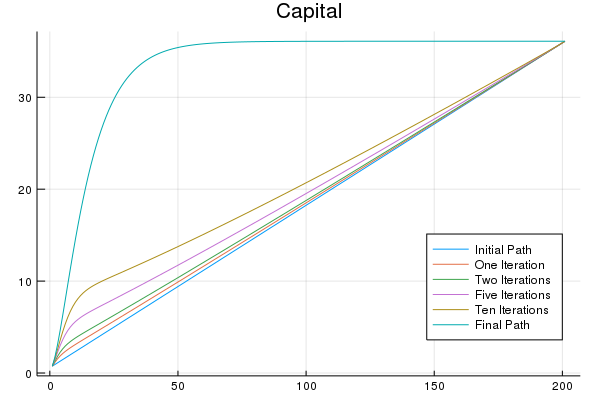
\includegraphics[scale=0.3]{p1_k.png}
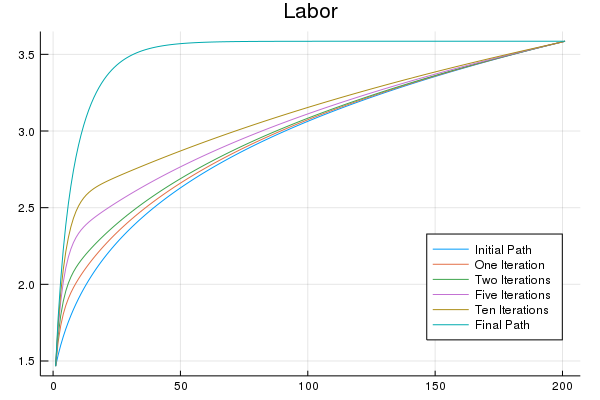
\includegraphics[scale=0.3]{p1_l.png}

\subsection{Part D}

I now solve for the optimal paths of output, employment, investment, consumption, and the real interest rate. Output is given by
\[  y_t = A k_t^\theta * l_t^{1-\theta}\]
investment is given by
\[ x_t = k_{t+1} - (1-\delta) k_t \]
consumption is given by
\[ c_t = y_t - x_t \]
and the real interest rate is given by
\[ r_t = MPK_t - \delta = \frac{\partial y_t}{\partial k_t} - \delta = \theta A \left(\frac{k_t}{l_t}\right)^{\theta - 1} - \delta \]
Employment is given by the optimal amount of labor, solved for above.

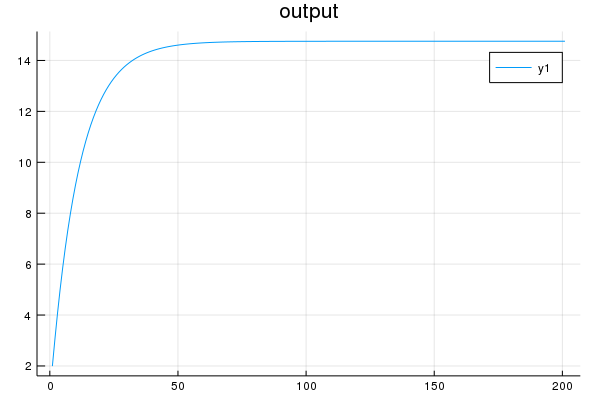
\includegraphics[scale=0.3]{p1_y.png}
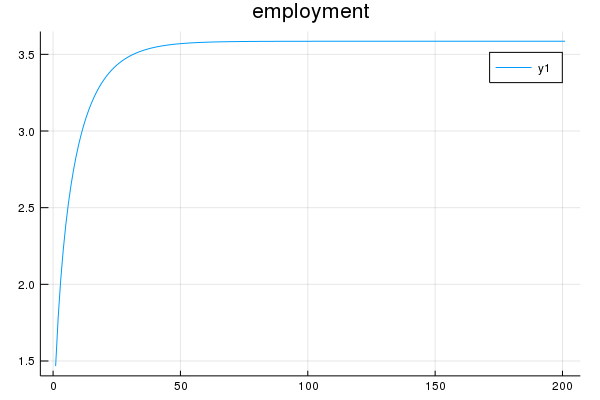
\includegraphics[scale=0.3]{p1_n.png}

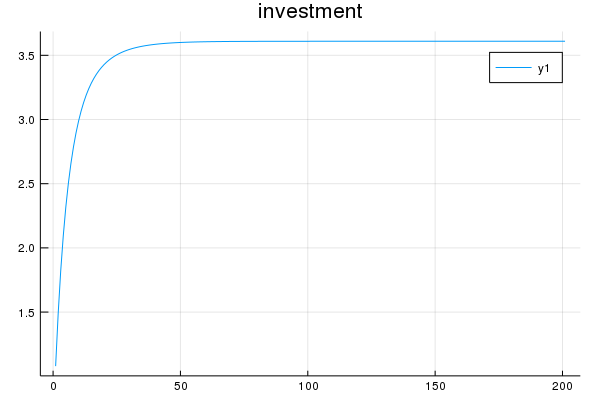
\includegraphics[scale=0.3]{p1_x.png}
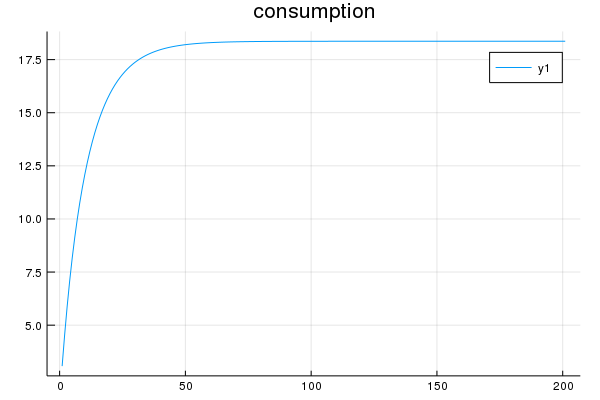
\includegraphics[scale=0.3]{p1_c.png}

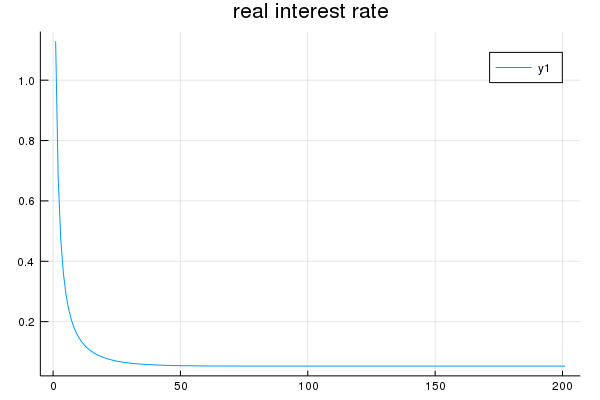
\includegraphics[scale=0.3]{p1_r.png}

\section{Question 2}

\subsection{Part A}

In this experiment, we begin with \(k_0 = k^*\) and calculate the optimal paths of capital and labor during a technology shock using the extended path method. My implementation solves this problem in about \(1.3\) seconds and needs \(660\) iterations.

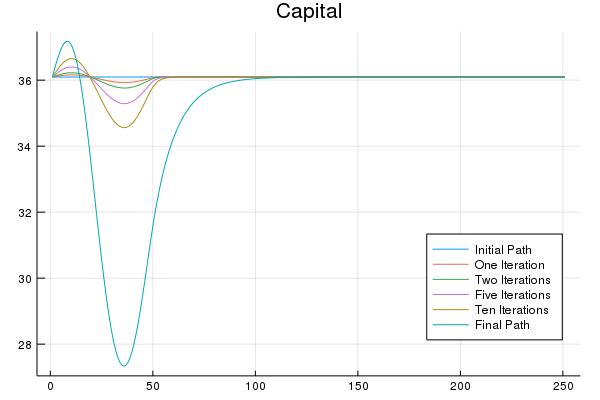
\includegraphics[scale=0.3]{p2_k}
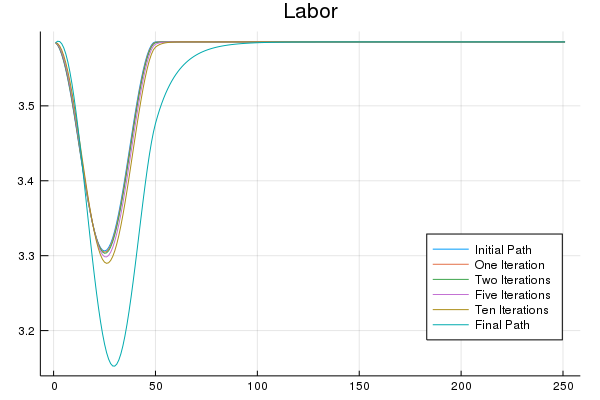
\includegraphics[scale=0.3]{p2_l}

\subsection{Part B}

I now solve for the paths of output, employment, investment, consumption, and the real interest rate during the recession. The first four drop immediately upon the impact of the technology shock. While capital increases on impact, because labor accounts for \(70\%\) of output under our calibration, output still falls upon the impact of the technology shock. For the same reason, labor decreases less than consumption (percentage-wise) during the recession.

The real interest rate first decreases because the increase in capital and the decrease in labor both decrease the marginal product of capital. However, as capital begins to go down in the middle of the recession, the real interest rate begins to rise instead. The decreasing part of the graph represents a period where more people want to save by holding capital, and thus the real interest rate does not need as high as before to induce savings. However, as output goes down and thus people save less (in gross terms) because they have less income, the interest rate increases to compensate.

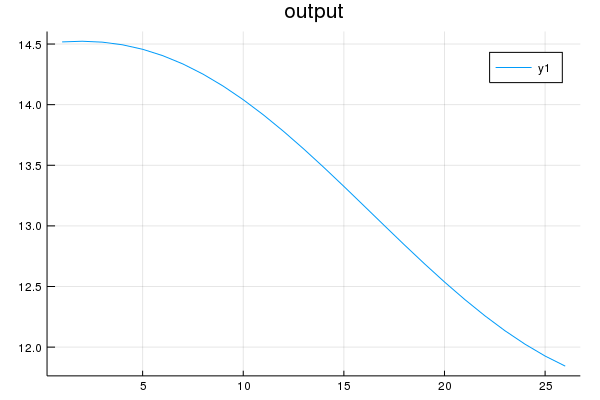
\includegraphics[scale=0.3]{p2_y.png}
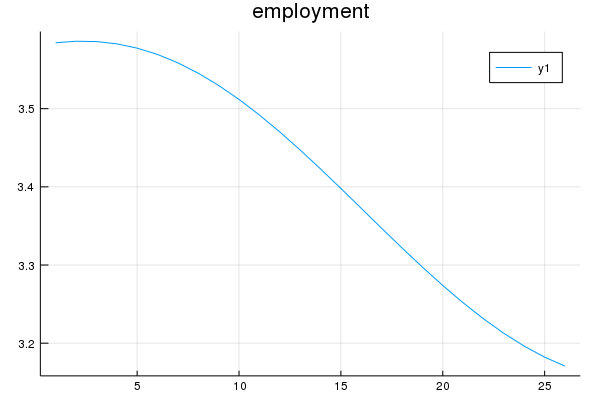
\includegraphics[scale=0.3]{p2_n.png}

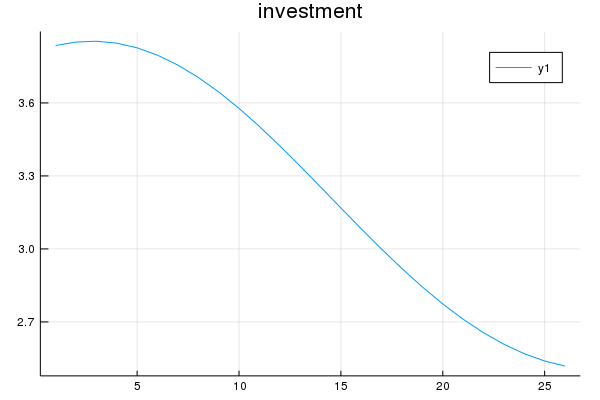
\includegraphics[scale=0.3]{p2_x.png}
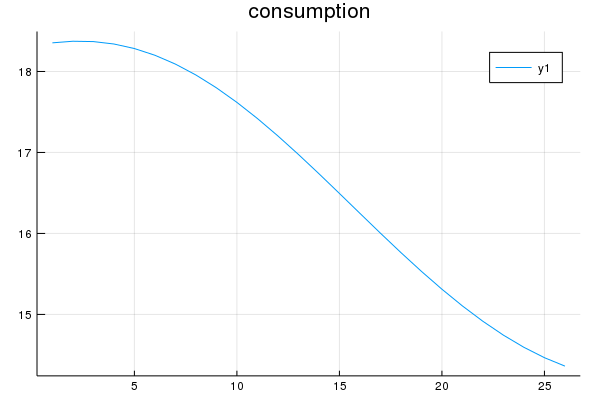
\includegraphics[scale=0.3]{p2_c.png}

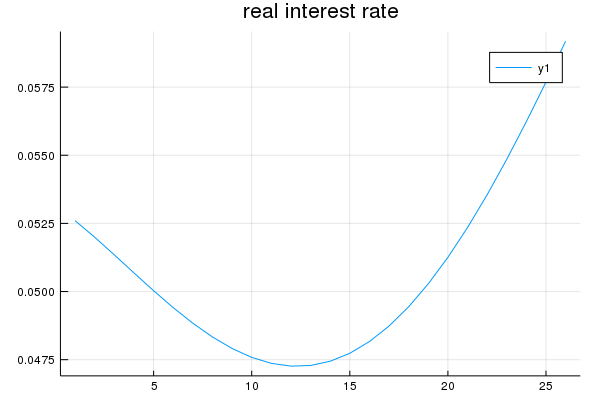
\includegraphics[scale=0.3]{p2_r.png}

\subsection{Part C}

The model is most successful in matching the trends of investment and employment. Total investment drops by about a third in the data as opposed to about a quarter in the model, and displays a monotonically decreasing drop throughout the recession. Employment displays a similar small but (approximately) monotonic decrease during the recession. By contrast, consumption decreases far too much in the model - consumption drops by about one-sixth in the model as opposed to a small decrease of less than \(3\%\) in the data. Furthermore, the real interest rate in the model increases before the end of the recession, while the effective federal funds rate is approximately monotonically decreasing throughout the entire recession. (Percentages were obtained by examining the value of each time series at the beginning and end of the recession in FRED and in the data produced by the model.)
\newline

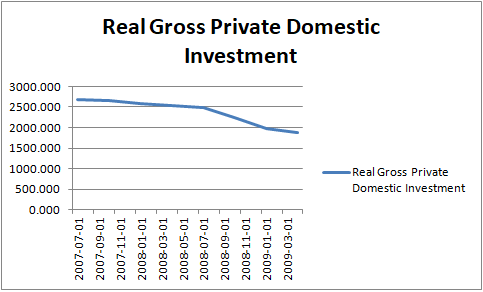
\includegraphics[scale=0.5]{rgpdi.png}
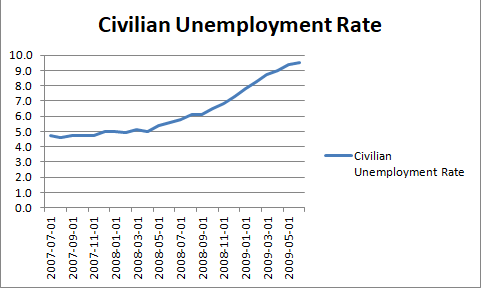
\includegraphics[scale=0.5]{cur.png}

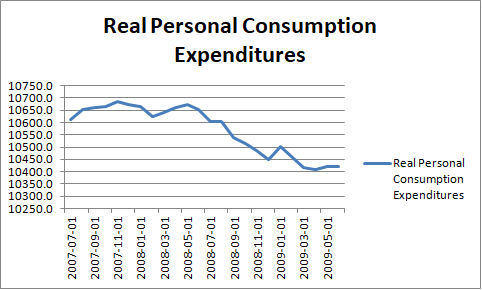
\includegraphics[scale=0.5]{rpce.png}
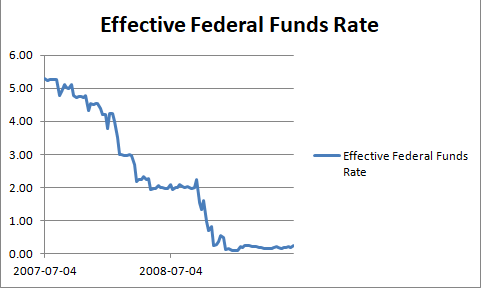
\includegraphics[scale=0.5]{effr.png}


I use the civilian unemployment rate because the employment rate is \(1-u\), taking the unemployment rate to be \(u\). By definition the employment rate should display the same dynamics as employment.

\newpage

\appendix

I provide my \texttt{Julia} code below.

\begin{lstlisting}[breaklines]
#Given parameters
const sigma = 1.5
const beta = 0.95
const theta = 0.3
const delta = 0.1

#Tolerance and step size for iteration algorithms
const tol = 0.00001
const h = 0.00000001

#Write steady-state A,k,l closed-form
const A = (1/(theta*beta*((1-theta)^((1-theta)/(1+theta)))))^((1+theta)/2)
const k_ss = (1-beta*(1-delta))^(-((1+theta)/(1-theta)))
const l_ss = (((1-theta)/(beta*theta))^0.5) * (1-beta *(1-delta))^(theta/(theta-1))

#Write the initial paths for capital; _c represents cycles
init_path = collect(range(0.75, length=201, stop=k_ss))
init_path_c = collect(range(k_ss, length=251, stop=k_ss))

#Write functions for labor and capital
#In every function of multiple capital values, k_m = k_t, k_t = k_{t+1}, and k_p = k_{t+2}, where the LHS is the Julia representation and the RHS is the TeX representation.

l(k,A_t) = ((1-theta)*A_t)^(1/(1+theta)) * (k^(theta/(1+theta)))
euler(k_t, k_m, k_p, A_m, A_t) = (beta * (theta*A_t * (k_m/l(k_m, A_m))^(theta-1) + (1-delta)))^(1/sigma) * (A_m * k_m^theta * l(k_m, A_m)^(1-theta) + (1-delta) * k_m - k_t - 0.5*(l(k_m,A_m))^2) - (A_t * k_t^theta * (l(k_t, A_t))^(1-theta) + (1-delta) * k_t - k_p - 0.5*(l(k_t, A_t))^2)

#Functions to get macro variables from capital array

x(k_m, k_t) = k_t - (1-delta) * k_m
y(k,A_t) = A_t * k^theta * l(k, A_t)^(1-theta)
c(k_m, k_t, A_m) = y(k_m,A_m) - x(k_m, k_t)
r(k,A_t) = theta*A*(k/l(k, A_t))^(theta-1) - delta

#create technology vectors
function A_cycle(t::Number)
    local A_ret
    if t < 51
        A_ret = A * (1 + 0.05 * (cos(pi * 0.04*t ) - 1))
    else
        A_ret = A
    end
    return A_ret
end

A_vec = zeros(201)
A_c_vec = zeros(251)

for t=1:length(A_vec)
    A_vec[t] = A
end

for t=1:length(A_c_vec)
    A_c_vec[t] = A_cycle(t)
end


#Root-finding methods modified for Problem 1 Part B

#Bisection method accepts a function (the euler equation), left and right endpoints a and b, fixed k_t and k_{t+2} (for the Euler equation), fixed A_t and A_{t+1}, and the pre-defined tolerance
function bisection_b(f::Function, a::Number, b::Number, k_m :: Number, k_p :: Number, A_m::Number, A_t::Number, tol::AbstractFloat)
    #Get values at endpoints
    p1 = f(a, k_m, k_p, A_m, A_t)
    p2 = f(b, k_m, k_p, A_m, A_t)

    #Initialize iteration tracker and midpoint
    i = 0
    local m

    #Loop until convergence
    while abs(b-a) > tol
        #find midpoint
        m = 0.5*(a+b)
        #print midpoint at each iteration
        println(m, ", i = ", i)
        println(" ")
        #get value at midpoint
        p3 = f(m, k_m, k_p, A_m, A_t)
        #kill bisection if solution is exact
        if p3 == 0
            break
        #check if left or right endpoint should be replaced
        elseif p1*p3 > 0
            a = m
            p1 = p3
        else
            b = m
            p2 = p3
        end
        i = i + 1
    end
    #return midpoint and number of iterations
    return m, i-1
end

#Newton's method accepts the Euler equation, an initial value of capital, k_t and k_{t+2}, A_t and A_{t+1}, a step size h, and the predefined tolerance
function Newton_b(f::Function, k_0::Number, k_m::Number, k_p::Number, A_m::Number, A_t::Number, h::Number, tol::AbstractFloat)
    #initialize iteration tracker and next capital
    i=0
    local k_1
    #print initial capital
    println(k_0, ", i = 0")
    println(" ")
    #run while loop until broken inside
    while true
        #Do Newton's method
        k_1 = k_0 - h*f(k_0, k_m, k_p, A_m, A_t)/(f(k_0 + h, k_m, k_p, A_m, A_t) - f(k_0, k_m, k_p, A_m, A_t))
        #Increase iterations
        i = i + 1
        # break if convergence is found
        if abs(k_1 - k_0 < tol)
            break
        end
        #if no convergence if found, replace the initial capital and start over
        k_0 = k_1
        println(k_0, ", i = ", i)
        println(" ")

    end
    #return the new capital and number of iterations
    return k_1, i
end

#Extended path method modified for Problem 1 Part C
function ext_path_1c(f::Function, path::Array{Float64,1}, A_path::Array{Float64,1}, h::AbstractFloat, tol::AbstractFloat)
    # initialize the new path
    local iter_path = zeros(length(path))
    #Initialize a number to keep track of whether every k has converged
    local stop_iter = 0
    #Initialize a number to keep track of iterations
    local i = 0

    #initialize paths at different iterations for part C
    local path_0 = path
    local path_1
    local path_2
    local path_5
    local path_10

    #run while some value of capital has not converged
    while stop_iter == 0
        #Set the first and last values of the iteration path to k_0 and k_ss
        iter_path[1] = path[1]
        iter_path[length(path)] = path[length(path)]

        #Find intermediate capital values by Newton's method; accept old k_{t+2} and new k_t to find k_{t+1}
        for j=1:(length(path) - 2)
            iter_path[j+1] = Newton(f, iter_path[j], iter_path[j], path[j+2], A_path[j], A_path[j+1], h, tol)[1]
        end
        #Add 1 to the stopper for each value which converged
        for j=1:length(path)
            if abs(iter_path[j] - path[j]) < tol
                stop_iter = stop_iter + 1
            end
        end

        #reset the stopper and the old path if convergence has not been found
        if stop_iter < length(path)
            stop_iter = 0
            path = iter_path
            #necessary because Julia will not let me overwrite iter_path unless it is a zero vector again
            iter_path = zeros(length(path))
        end

        # increase number of iterations and spit out the paths at specified number of iterations
        i = i + 1
        if i==1
            path_1 = path
        elseif i==2
            path_2 = path
        elseif i==5
            path_5 = path
        elseif i==10
            path_10 = path
        end
    end
    #return all the paths and the number of iterations
    return path_0, path_1, path_2, path_5, path_10, iter_path, i
end

#Generalized root finding and extended path
#Bisection method accepts a function (the euler equation), left and right endpoints a and b, fixed k_t and k_{t+2} (for the Euler equation), fixed A_t and A_{t+1}, and the pre-defined tolerance
function bisection(f::Function, a::Number, b::Number, k_m :: Number, k_p :: Number, A_m::Number, A_t::Number, tol::AbstractFloat)
    #Get values at endpoints
    p1 = f(a, k_m, k_p, A_m, A_t)
    p2 = f(b, k_m, k_p, A_m, A_t)

    #Initialize iteration tracker and midpoint
    i = 0
    local m

    #Loop until convergence
    while abs(b-a) > tol
        #increase number of iterations, find midpoint, get value at midpoint
        m = 0.5*(a+b)
        p3 = f(m, k_m, k_p, A_m, A_t)
        #kill bisection if solution is exact
        if p3 == 0
            break
        #check if left or right endpoint should be replaced
        elseif p1*p3 > 0
            a = m
            p1 = p3
        else
            b = m
            p2 = p3
        end
        i = i + 1
    end
    #return midpoint and number of iterations
    return m, i-1
end

#Newton's method accepts the Euler equation, an initial value of capital, k_t and k_{t+2}, A_t and A_{t+1}, a step size h, and the predefined tolerance
function Newton(f::Function, k_0::Number, k_m::Number, k_p::Number, A_m::Number, A_t::Number, h::Number, tol::AbstractFloat)
    #initialize iteration tracker and next capital
    i=0
    local k_1
    #run while loop until broken inside
    while true
        #Do Newton's method
        k_1 = k_0 - h*f(k_0, k_m, k_p, A_m, A_t)/(f(k_0 + h, k_m, k_p, A_m, A_t) - f(k_0, k_m, k_p, A_m, A_t))
        #Increase iterations
        i = i + 1
        # break if convergence is found
        if abs(k_1 - k_0 < tol)
            break
        end
        #if no convergence if found, replace the initial capital and start over
        k_0 = k_1

    end
    #return the new capital and number of iterations
    return k_1, i
end

#Extended path method modified for Problem 1 Part C
function ext_path(f::Function, path::Array{Float64,1}, A_path::Array{Float64,1}, h::AbstractFloat, tol::AbstractFloat)
    # initialize the new path
    local iter_path = zeros(length(path))
    #Initialize a number to keep track of whether every k has converged
    local stop_iter = 0
    #Initialize a number to keep track of iterations
    local i = 0

    #run while some value of capital has not converged
    while stop_iter == 0
        #Set the first and last values of the iteration path to k_0 and k_ss
        iter_path[1] = path[1]
        iter_path[length(path)] = path[length(path)]

        #Find intermediate capital values by Newton's method; accept old k_{t+2} and new k_t to find k_{t+1}
        for j=1:(length(path) - 2)
            iter_path[j+1] = Newton(f, iter_path[j], iter_path[j], path[j+2], A_path[j], A_path[j+1], h, tol)[1]
        end
        #Add 1 to the stopper for each value which converged
        for j=1:length(path)
            if abs(iter_path[j] - path[j]) < tol
                stop_iter = stop_iter + 1
            end
        end

        #reset the stopper and the old path if convergence has not been found
        if stop_iter < length(path)
            stop_iter = 0
            path = iter_path
            #necessary because Julia will not let me overwrite iter_path unless it is a zero vector again
            iter_path = zeros(length(path))
        end

        # increase number of iterations
        i = i + 1
    end
    #return the path and the number of iterations
    return iter_path, i
end


#function to calculate paths of various macro parameters from capital array; accepts capital and technology. Special for part d: technology treated as constant

function macrovars(path::Array{Float64,1}, A_path::Array{Float64,1})
    local n_path = zeros(length(path))
    local x_path = zeros(length(path))
    local c_path = zeros(length(path))
    local y_path = zeros(length(path))
    local r_path = zeros(length(path))

    for t=1:length(path)
        #find investment and consumption
        if t ≠ length(path)
            x_path[t] = x(path[t], path[t+1])
            c_path[t] = c(path[t], path[t+1], A_path[t])
        #At last value accept steady-state capital twice because k_{t+1} = k_t = k ∀t
        else
            x_path[t] = x(path[t], path[t])
            c_path[t] = c(path[t], path[t], A_path[t])
        end

        #find employment
        n_path[t] = l(path[t], A_path[t])
        #find output
        y_path[t] = y(path[t],A_path[t])
        #find interest rate
        r_path[t] = r(path[t], A_path[t])
    end

    return n_path, x_path, c_path, y_path, r_path
end

function l_convert(k_path::Array{Float64,1}, A_path::Array{Float64,1})
    local l_path = zeros(length(k_path))
    for t=1:length(k_path)
        l_path[t] = l(k_path[t], A_path[t])
    end
    return l_path
end

#get the bisection solution
#time calculated without the printing
sol = bisection_b(euler,1,1.4,0.85,0.95, A, A, tol)
@time bisection(euler,1,1.4,0.85,0.95, A, A, tol)

#get the newton solution
sol2 = Newton_b(euler, 0.85, 0.85, 0.95, A, A, h, tol)
@time Newton(euler, 0.85, 0.85, 0.95, A, A, h, tol)

#do the extended path
sol_paths = ext_path_1c(euler, init_path, A_vec, h, tol)
@time ext_path(euler, init_path, A_vec, h, tol)
paths = [sol_paths[1], sol_paths[2], sol_paths[3], sol_paths[4], sol_paths[5], sol_paths[6]]

l_paths = [l_convert(paths[1], A_vec), l_convert(paths[2], A_vec), l_convert(paths[3], A_vec), l_convert(paths[4], A_vec), l_convert(paths[5], A_vec), l_convert(paths[6], A_vec)]
macro_paths = macrovars(sol_paths[6], A_vec)

#initialize plotting
using Plots

#plot the vectors
plot_k = plot(paths, title="Capital", label=["Initial Path" "One Iteration" "Two Iterations" "Five Iterations" "Ten Iterations" "Final Path"], legend=:bottomright)
savefig("p1_k")
plot_l = plot(l_paths, title="Labor", label=["Initial Path" "One Iteration" "Two Iterations" "Five Iterations" "Ten Iterations" "Final Path"], legend=:bottomright)
savefig("p1_l")

plot_n = plot(macro_paths[1], title="employment")
savefig("p1_n")
plot_x = plot(macro_paths[2], title="investment")
savefig("p1_x")
plot_c = plot(macro_paths[4], title="consumption")
savefig("p1_c")
plot_y = plot(macro_paths[3], title="output")
savefig("p1_y")
plot_r = plot(macro_paths[5], title="real interest rate")
savefig("p1_r")

#path_p1_macro_plot = plot(plot_n, plot_x, plot_c, plot_y, plot_r, layout=(length(macro_paths),1),legend=false)

#do problem 2
sol_p2 = ext_path_1c(euler, init_path_c, A_c_vec, h, tol)

k_p2 = [sol_p2[1], sol_p2[2], sol_p2[3], sol_p2[4], sol_p2[5], sol_p2[6]]
l_p2 = [l_convert(sol_p2[1], A_c_vec), l_convert(sol_p2[2], A_c_vec), l_convert(sol_p2[3], A_c_vec), l_convert(sol_p2[4], A_c_vec), l_convert(sol_p2[5], A_c_vec), l_convert(sol_p2[6], A_c_vec)]
sol_p2_macro = macrovars(sol_p2[6], A_c_vec)



#initialize the macro variable vectors so we can truncate
x_vec = zeros(26)
y_vec = zeros(26)
c_vec = zeros(26)
n_vec = zeros(26)
r_vec = zeros(26)

#truncate the macro variables
for t=1:26
    x_vec[t] = sol_p2_macro[2][t]
    y_vec[t] = sol_p2_macro[3][t]
    c_vec[t] = sol_p2_macro[4][t]
    r_vec[t] = sol_p2_macro[5][t]
    n_vec[t] = sol_p2_macro[1][t]
end

#plot the vectors
plot_k2 = plot(k_p2, title="Capital", label=["Initial Path" "One Iteration" "Two Iterations" "Five Iterations" "Ten Iterations" "Final Path"], legend=:bottomright)
savefig("p2_k")
plot_l2 = plot(l_p2, title="Labor", label=["Initial Path" "One Iteration" "Two Iterations" "Five Iterations" "Ten Iterations" "Final Path"], legend=:bottomright)
savefig("p2_l")

plot_n2 = plot(n_vec, title="employment")
savefig("p2_n")
plot_x2 = plot(x_vec, title="investment")
savefig("p2_x")
plot_c2 = plot(c_vec, title="consumption")
savefig("p2_c")
plot_y2 = plot(y_vec, title="output")
savefig("p2_y")
plot_r2 = plot(r_vec, title="real interest rate")
savefig("p2_r")

\end{lstlisting}

\end{document}
